\chapter{Modelos continuos en epidemiología}

Los modelos continuos, al igual que los discretos, tratan de describir la evolución y desarrollo de una enfermedad a lo largo del tiempo. La diferencia con los modelos discretos es que, al contrario que en estos, el tiempo se supone continuo.

Mientras en los modelos discretos consideramos un $\Delta t$ que hace referencia a los incrementos del tiempo entre dos valores consecutivos de la cantidad de individuos de cada estado, en los modelos continuos el tiempo se supone continuo, y por tanto no se trabaja con una cantidad numerable de valores.

\section{Tipos de modelos}

Al igual que los modelos discretos, los modelos continuos (principalmente SI, SIR y SIS) usan los estados Susceptible, Infectado y Recuperado. Los nombres suelen hacer referencia al flujo que se sigue para pasar entre los estados. Así, por ejemplo un modelo SI pasa de susceptible a infectado, uno SIR de susceptible a infectado y recuperado y SIS alterna entre susceptible e infectado.

En estos modelos se hacen dos suposiciones:
\begin{enumerate}
\item La población se mezcla de manera homogénea, es decir, todos los individuos tienen la misma probabilidad de contraer la enfermedad.
\item El total de la población es constante y lo denotaremos por $N$.
\end{enumerate}

En este capítulo estudiaremos los principales modelos epidemiológicos continuos análogos a los estudiados en el capítulo anterior.


\section{Modelo SI continuo}

Expresando $\alpha$ como una tasa podemos obtener las ecuaciones diferenciales análogas de la siguiente manera. Considerando

$$\frac{S_{n+1} - S_n}{\Delta t} \approx S'(t),$$

El análogo continuo al sistema \eqref{eqn: SI} viene dado por:

\begin{equation}
\label{eqn:SI_continuo}
\begin{aligned}
S'(t) & = -\frac{\alpha}{N}SI \\
I'(t) & = \frac{\alpha}{N}SI
\end{aligned}
\end{equation}

con condiciones iniciales $S(0)+I(0)=N$.

De \eqref{eqn:SI_continuo} se puede ver que $I'>0$ y $S'<0$, luego ambas funciones son estrictamente monótonas, al igual que el modelo discreto.

Calculamos los puntos de equilibrio de manera análoga al caso discreto, es decir, suponemos que las funciones son constantes y, resolviendo el sistema de ecuaciones, podemos comprobar que las soluciones convergen a $(S^*,I^*)=(0,N)$ y, por tanto, tienen el mismo comportamiento que en el caso discreto.

Sustituyendo en el modelo $S=N-I$ obtenemos la ecuación diferencial logística continua

$$I' = \frac{\alpha}I{N}(N-I).$$

Esta ecuación diferencial se puede resolver por separación de variables como sigue:

\begin{equation}
\begin{aligned}
I'=\frac{\alpha}{N}I(N-I) & \Leftrightarrow \int \frac{dI}{I(N-I)} = \int \frac{\alpha}{N} dt \\
& \Leftrightarrow \frac{1}{N}\int \left(\frac{1}{I}+\frac{1}{N-I}\right) dI = \frac{\alpha}{N}t+c \\
& \Leftrightarrow  \frac{1}{N}\log{\frac{I}{N-I}} = \frac{\alpha}{N}t+c \\
& \Leftrightarrow  \frac{I}{N-I} = Ae^{\alpha t} \\
& \Leftrightarrow  I = Ae^{\alpha t}(N-I) \\
& \Leftrightarrow  I(1+Ae^{\alpha t}) = Ae^{\alpha t}N \\
& \Leftrightarrow  I(t) = \frac{Ae^{\alpha t}N}{1+Ae^{\alpha t} }
\end{aligned}
\end{equation}

Usando el valor inicial $I(0)=I_0$ tenemos:

\begin{equation}
\begin{aligned}
I_0 = I(0) = \frac{AN}{1+A} & \Leftrightarrow (1+A)I_0 = AN \\
& \Leftrightarrow A(N-I_0) = I_0 \\
& \Leftrightarrow A = \frac{I_0}{N-I_0}
\end {aligned}
\end{equation}

luego la solución general es:

$$I(t) = \frac{I_0e^{\alpha t}N}{(N-I_0)+I_0e^{\alpha t}} = \frac{I_0N}{(N-I_0)e^{-\alpha t}+I_0}.$$

Es claro que $I$ tiende monótonamente a $N$, luego tiene el mismo comportamiento que el modelo discreto.


\section{Modelo SIS continuo}

El modelo continuo correspondiente al modelo SIS se comporta de la misma forma que el modelo discreto, y viene expresado por:

\begin{equation}
\label{eqn: modelo_SIS_continuo}
\begin{aligned}
S'(t) = & -\frac{\alpha}{N}SI+\gamma I \\
I'(t) = & I\left( \frac{\alpha}{N}S-\gamma \right) \\
\end{aligned}
\end{equation}

donde $S(0)+I(0)=N$.

Si $\mathcal{R}_{SIS}\leq 1$ entonces no ocurre una epidemia, y si $\mathcal{R}_{SIS} > 1$ entonces hay una epidemia.

\textcolor{red}{Completar. Pongo alguna grafiquita o algo?}



\section{Modelo SIR continuo}


El modelo continuo correspondiente al modelo SIR se comporta de la misma forma que el modelo discreto, y viene expresado por:

\begin{equation}
\label{eqn: modelo_SIR_continuo}
\begin{aligned}
S'(t) = & -\dfrac{\alpha}{N}SI \\
I'(t) = & I\left(\dfrac{\alpha}{N}S-\gamma \right) \\
R'(t) = & \gamma I
\end{aligned}
\end{equation}

donde $S(0)+I(0)+R(0)=N$. El número básico reproductivo en este caso se define como
$$\mathcal{R}_{SIR}=\frac{S(0)\alpha }{N\gamma },$$
y si como hemos visto $\mathcal{R}_{SIR}\leq 1$  se dice que no hay epidemia, pero en cambio, si es mayor, se dice que sí la hay.

\section{Modelo Kermack-McKendrick}

La información para el desarrollo de esta sección se ha obtenido principalmente de \cite{brauerMathematicalModelsPopulation2012}.

El modelo de Kermack-McKendrick es un modelo sencillo basado en suposiciones simples en el flujo de la población de unos grupos a otros según su estado respecto a la enfermedad. Estos grupos son susceptibles, infectados y recuperados, inmunizados o fallecidos.

Este modelo es, por tanto, una modificación del modelo SIR ya estudiado. La diferencia con el modelo SIR ya estudiado es que en este modelo se supone que un individuo infectado hace contacto suficiente para contagiar la enfermedad con $\alpha N$ individuos por unidad de tiempo, mientras en el modelo SIR se supone que $\alpha$ es el número medio de individuos con los que un infectado tiene suficiente contacto para contagiarlo en una unidad de tiempo.

El modelo se describe como:

\begin{equation}
\label{eqn: KMK}
\begin{aligned}
S' & = -\alpha SI \\
I' & = \alpha SI - \gamma I \\
R' & = \gamma I
\end{aligned}
\end{equation}

Las suposiciones en las que se basa el modelo descrito son:

\begin{itemize}
\item Un individuo hace contacto suficiente para contagiar la enfermedad con $\alpha N$ individuos por unidad de tiempo, sienod $N$ el total de la población.
\item Los infectados pasan a recuperados, inmunizados o fallecidos con la tasa $\gamma I$ por unidad de tiempo.
\item La población total es constante, no hay incorporaciones ni salidas.
\item No se consideran fallecimientos como grupo aparte, así la población es constante.
\end{itemize}

\begin{figure}
\begin{center}
\caption{Esquema del modelo de Kermack-McKendrick y modelo SIR}
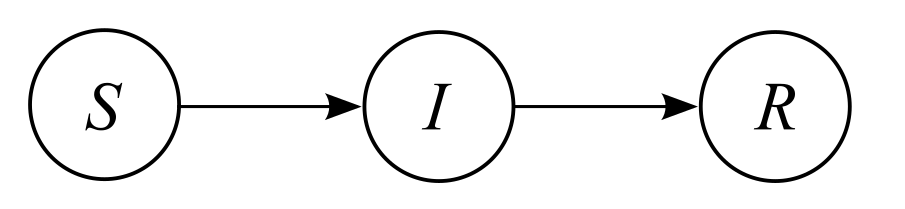
\includegraphics[scale=0.5]{esquema_sir}
\end{center}
\end{figure}

De acuerdo con la primera suposición, dado que la probabilidad de que aleatoriamente el contacto de un infectado sea con un individuo susceptible es $\frac{S}{N}$, el número de nuevos infectados por unidad de tiempo por infectado es $\frac{\alpha NS}{N}$, dando lugar a una tasa de nuevos infectados de $\frac{\alpha  N S I}{N}=\alpha SI$. Notemos que ambas aproximaciones dan lugar a la misma tasa de nuevos infectados.

Observemos también que, al igual que en el modelo SIR, se cumple $N=S+I+R$.

Para la tercera suposición consideramos el grupo de individuos que fueron infectados en un mismo momento, y sea $u(s)$ el conjunto de estos que aún son infecciosos $s$ unidades de tiempo después de haber sido infectados. Si una porción $\gamma$ de estos deja de pertenecer a la clase de individuos infectados por unidad de tiempo, entonces

$$u'=-\gamma u,$$

y la solución de esta ecuación diferencial es

$$u(s)=u(0)e^{-\gamma s}.$$

Por tanto, la fracción de infectados que siguen estando en la clase infectados $s$ unidades de tiempo después de haberse convertido en infectados es $e^{-\gamma s}$, luego la duración del período infeccioso se distribuye según una exponencial, con significado
$$\int_0^\infty e^{-\gamma s}ds=1/\gamma,$$
y esto es lo que la segunda suposición realmente significa. Si en lugar de suponer esto, suponemos que la fracción de infectados que permanecen infectados en un tiempo $\tau$ después de haberse infectado es $P(\tau )$, la segunda ecuación de \eqref{eqn: KMK} se reemplaza por:

$$I(t)=I_0(t)+\int_0^\infty \alpha S(t-\tau )I(t-\tau )P(\tau ) d\tau ,$$

donde $I_0(t)$ hace referencia a los miembros de la población que eran infectados en el instante inicial y siguen siendo infecciosos en el momento $t$.

Las suposiciones de que la tasa de contactos es proporcional al tamaño de la población $N$ con una constante de proporcionalidad constante $\alpha$ y de una distribución exponencial de tasa de recuperación son demasiado simples para ser realistas. Existen otros modelos más generales que se pueden analizar, pero finalmente muchos modelos más realistas muestran comportamientos similares a estos modelos más simples.

En nuestro modelo \eqref{eqn: KMK}, $R$ se determina una vez que se conocen $S$ e $I$, pero podemos eliminar la tercera ecuación del modelo, dejando este formado solamente por dos ecuaciones:

\begin{equation}
\label{eqn: KMK_sinR}
\begin{aligned}
S' & = -\alpha SI, \\
I' & = (\alpha S - \gamma ) I,
\end{aligned}
\end{equation}

junto con las condiciones iniciales:
$$S(0)=S_0, \quad I(0)=I_0, \quad S_0+I_0=N.$$

El modelo solo tiene sentido si $S(t)$ e $I(t)$ se mantienen no negativos, luego si alguno de los dos llega a $0$, consideramos que el estudio ha terminado.

\begin{lemma}
Dado el modelo \eqref{eqn: KMK_sinR}, se tiene que $S'<0$ para todo $t$, y además $I'>0$ si, y solo si, $S>\frac{\gamma}{\alpha}$.
\end{lemma}

Es decir, $I$ aumenta mientras se cumpla que $S>\frac{\gamma}{\alpha}$, pero como $S$ decrece para todo $t$, finalmente se tiene que $S<\frac{\gamma}{\alpha}$, y por tanto $I$ deja de aumentar.

Si $S_0<\frac{\gamma}{\alpha}$, entonces $I$ decrece a $0$ y no hay una epidemia, mientras que si $S_0>\frac{\gamma}{\alpha}$, $I$ comienza creciendo hasta el máximo obtenido cuando $S=\frac{\gamma}{\alpha}$ y luego decrece hasta $0$, en cuyo caso hay una epidemia.

Definimos el número básico reproductivo como:

$$\mathcal{R}_{KMK}=\frac{\alpha S_0}{\gamma}.$$

De esta manera, si $\mathcal{R}_{KMK}<1$ no hay una epidemia, mientras si $\mathcal{R}_{KMK}>1$ hay una epidemia. 





\section{Análisis de los parámetros de los modelos}

\subsection{Introducción}

Estimar la tasa de transmisión media es uno de los aspectos más cruciales en epidemiología. Esta tasa condiciona la fase de la epidemia e incluso si va a extinguirse. Es combinación de tres factores:

\begin{enumerate}
\item Coeficiente de virulencia: Relacionado con el agente infeccioso.
\item Coeficiente de susceptibilidad: Relacionado con el anfitrión.
\item Número de contactos por unidad de tiempo entre individuos.
\end{enumerate}

Los dos primeros factores se tienen en cuenta a la vez en la probabilidad de transmisión.

Todos los factores pueden cambiar con el tiempo. El primero, debido a mutaciones del virus y los dos últimos por medidas de contención. Por tanto, observar el decrecimiento de la transmisión media en una enfermedad es una buena forma de comprobar la efectividad de las medidas de contención.

En el artículo \cite{demongeotSIEpidemicModel} se presenta un modelo SI modificado con el objetivo de compararlo con los datos obtenidos en la pandemia de la COVID-19 en China hasta el momento, y así tratar de predecir su comportamiento en el futuro.

El modelo SI continuo considerado es el siguiente:

\begin{equation}
\label{eqn: SI_cont}
\begin{aligned}
S'(t) = & -\tau (t)S(t)I(t) \\
I'(t) = & \tau (t)S(t)I(t) -vI(t)
\end{aligned}
\end{equation}

donde $S(t)$ es el número de individuos susceptibles , $I(t)$ el número de individuos infectados en el tiempo $t$ y $\tau (t)$ la tasa de transmisión, que combina el número de contactos por unidad de tiempo y la probabilidad de transmisión. Observemos que $\tau (t)$ se considera variable respecto al tiempo, al contrario que en el caso SI clásico estudiado antes. Además, notemos que $v$ es una constante, donde $1/v$ es la duración media del período de infección, y $vI(t)$ el flujo de individuos recuperados o fallecidos. %vI(t) es el flujo de recuperados o muertos porque ha mezclado el modelo SI y SIR; vI(t) serian los recuperados, pero se ahorra la ecuacion de la R

Se consideran las condiciones iniciales

$$S(t_0)=S_0>0, \: I(t_0)=I_0>0.$$

Ahora, consideramos que al final del período infeccioso nos han informado de una fracción del total de casos, en este caso la fracción la denotamos por $f\in (0,1]$. Sea $C_R(t)$ el número total acumulado de casos reportados. Entonces:

\begin{equation}
\label{eqn: acumulada}
C_R(t) = {C_R}_0 + vfC_I(t), \forall t \geq t_0
\end{equation}

donde $C_{R0}$ representa el número de casos reportados al inicio del estudio y 

$$C_I(t) = \int_{t_0}^t I(w) dw $$

siendo $C_I$ el número total de infectados acumulado.

Asumimos conocidos $S_0 > 0$, $1/v>0$, $f\in (0,1]$. Por tanto, queremos averiguar el número inicial de infectados $I_0$ y la tasa de transmisión $\tau (t)$.

\subsection{Aproximación de $I_0$ y $\tau (t_0)$}
Siguiendo \cite{demongeotSIEpidemicModel}, procedemos a intentar aproximar $I_0$ y $\tau (t_0)$:

Al comienzo de la pandemia podemos suponer que $S(t)$ y $\tau (t)$ son constantes e iguales a $S_0$ y $\tau_0 = \tau (t_0)$, respectivamente. Sustituyendo estos valores en la ecuación \eqref{eqn: SI_cont} obtenemos:

$$I'(t) = (\tau_0 S_0 -v) I(t).$$

Resolviendo la ecuación diferencial llegamos a:

$$I(t) = I_0\exp{((\tau_0 S_0-v)(t-t_0))}.$$

Sustituyendo en \eqref{eqn: acumulada}:

$$C_R(t) = {C_R}_0 + vfI_0\frac{\mathrm{e}^{(\tau_0 S_0 -v)(t-t_0)} -1}{\tau_0 S_0-v}.$$

De este modo, hemos obtenido un primer modelo para los casos acumulados al principio de la pandemia.

Reescribimos la ecuación anterior como:

\begin{equation}
\label{eqn: acumulada_modelo}
C_R(t) = \chi_1 \mathrm{e}^{\chi_2 t} -\chi_3.
\end{equation}

Estimamos $\chi_3$ usando los datos de la epidemia obtenidos, y el mejor ajuste para los datos se obtiene con $\chi_3=0$.

Ahora, usando \eqref{eqn: acumulada} y \eqref{eqn: acumulada_modelo} tenemos:

\begin{equation}
I_0=\frac{\chi_1\chi_2\mathrm{e}^{\chi_2 t_0}}{vf}
\end{equation}

Y, como sabemos que $\chi_2 = \tau_0 S_0-v$, entonces

\begin{equation}
\tau_0 = \frac{\chi_2+v}{S_0}.
\end{equation}

Si suponemos $\tau (t) = \tau_0$ constante, tenemos que el modelo queda:

\begin{equation}
\begin{aligned}
S'(t) = -\tau_0S(t)I(t) \\
I'(t) = \tau_0S(t)I(t) -vI(t)
\end{aligned}
\end{equation}

Usando la ecuación de $S(t)$ y resolviéndola obtenemos:

$$S(t) = S_0\exp{\left( -\tau_0 \int_{t_0}^t I(w) dw \right)} = S_0\exp{(-\tau_0 C_I(t))}$$

Ahora, sustituyendo esta expresión en la ecuación de $I(t)$ del modelo y usando $C_I'(t)=I(t)$:

$$I'(t) = S_0\exp{\left( -\tau_0 C_I(t)\right) }\tau_0 C_I'(t)-vI(t)$$

Finalmente, integrando entre $t_0$ y $t$ tenemos que:

$$I(t)=C_I'(t)=I_0+S_0(1-\exp{(-\tau_0 C_I(t)}))-vC_I(t).$$
 
Observamos entonces que el número total acumulado de infectados es monótono creciente, ya que $I(t)>0$ siempre por positividad de las soluciones y $C_I'(t)=I(t)>0$. Cabe destacar que esto no implica que el número de infectados sea monótono creciente.

\begin{theorem}
Sea $t>t_0$ fijo. El número de infectados acumulados es estrictamente creciente respecto a las siguiente cantidades:
\begin{itemize}
\item $I_0>0$: Número inicial de infectados
\item $S_0>0$: Número inicial de individuos susceptibles.
\item $\tau>0$: Tasa de transmisión
\item $1/v$: Tiempo medio de la infección.
\end{itemize}
\end{theorem}

\subsection{Fórmula teórica para $\tau (t)$}

Usando la ecuación del modelo inicial \eqref{eqn: SI_cont} obtenemos:
% La ecuacion de la S$

$$S(t) = S_0 \exp{\left( - \int_{t_0}^t \tau(w) I(w) dw \right) } $$ 

Ahora, sustituyendo en la ecuación \eqref{eqn: SI_cont}:
% La ecuacion de la I

$$I'(t) = S_0 \exp{\left( - \int_{t_0}^t \tau(w) I(w) dw \right) } \tau (t) I(t) -vI(t) $$

Integramos en ambos lados entre $t_0$ y $t$, luego:

$$ C_I'(t) = I_0 + S_0 \left( 1-\exp{\left(- \int_{t_0}^t \tau (w) I(w)dw \right)}\right) -vC_I(t)$$

Equivalentemente, por \eqref{eqn: acumulada}:

$$C_R'(t) = vf\left( I_0 + S_0 \left( 1-\exp{\left(- \frac{1}{vf}\int_{t_0}^t \tau (w ) C_R'(w)dw \right)}\right)\right) +v{C_R}_0 -vC_R(t)$$

Así, obtenemos el Teorema 3.1 de \cite{demongeotSIEpidemicModel}, que nos da la relación directa buscada.







